\\
The relevant files for this section is the main.py and Q1.py

\subsection{}
\begin{figure*}[h!]
\centering
\begin{tabular}{cc}
    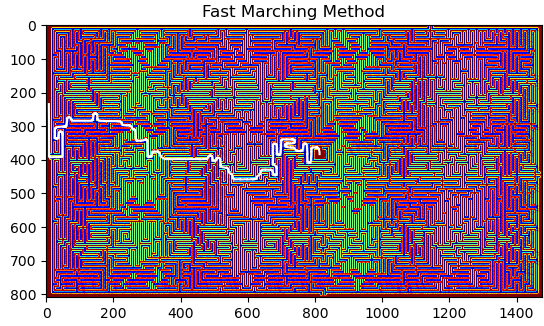
\includegraphics[width=0.45\linewidth]{figs/Ex1/Fast Marching Method.PNG} &
    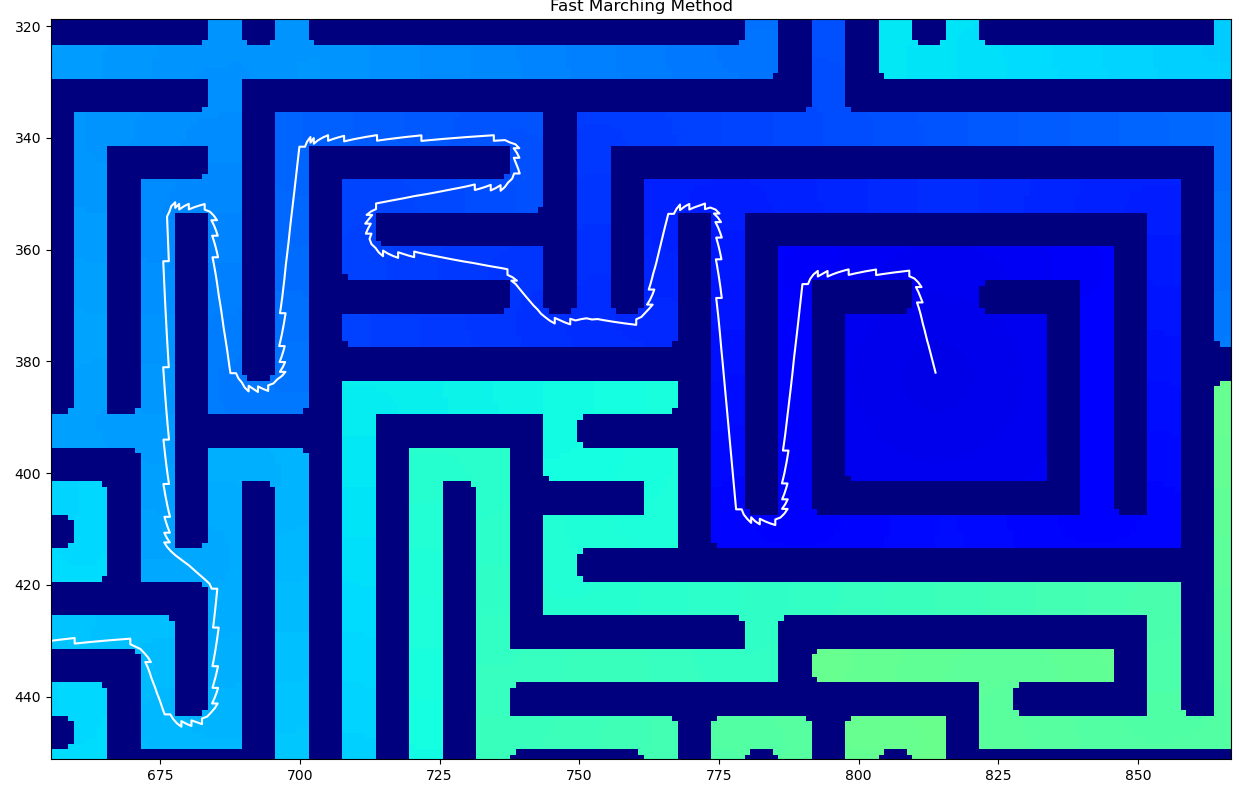
\includegraphics[width=0.45\linewidth]{figs/Ex1/Fast Marching Method_ZoomIn.PNG} 
\end{tabular}
\caption{\small Fast Marching Method}
 \label{fig:fmm}
\end{figure*}

\begin{figure*}[h!]
\centering
\begin{tabular}{cc}
    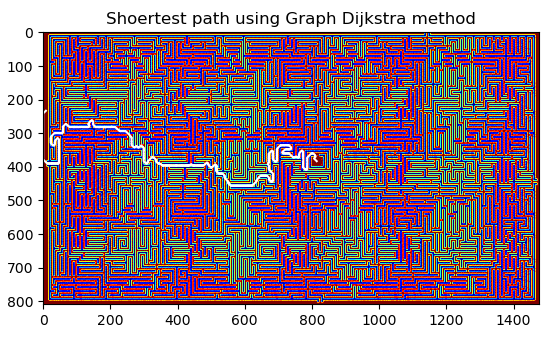
\includegraphics[width=0.45\linewidth]{figs/Ex1/Shoertest path using Graph Dijkstra method.PNG} &
    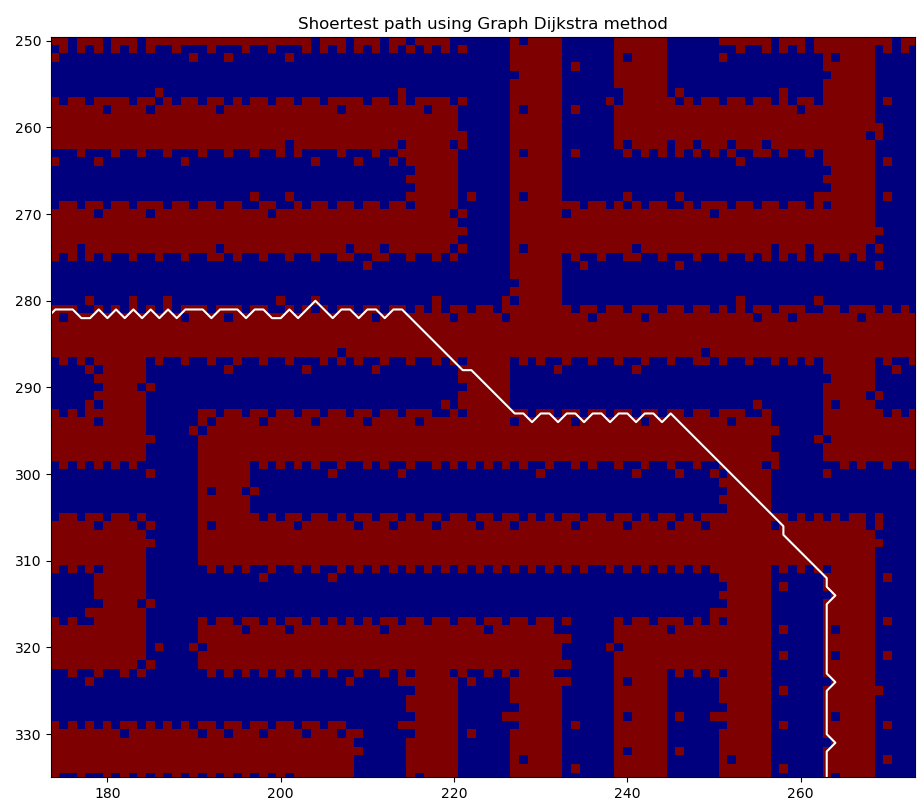
\includegraphics[width=0.45\linewidth]{figs/Ex1/Shoertest path using Graph Dijkstra method_ZoomIn.PNG} 
\end{tabular}
\caption{\small Graph connection using Dijkstra Method}
 \label{fig:dijkstra}
\end{figure*}
As can be seen both algorithms found the same shortest path, as we thought. But if we zoom in and take small segments, we can see some difference between the methods. FFM method path goes +/- in the middle of the maze path while the Dijkstra method goes along the walls and even between the discretization pixels. It can be explained by the fact the Dijkstra using graph connection and indeed the shortest path is along the walls. While the FFM using navigation through the maze derivation which means the path is more smooth and the stronger derivation is indeed in the middle between the walls.
\subsection{}
The velocity of light trough medium is the inverse of the refraction index. so we use the FFM by inverse the refraction indices. The results we got was different from the tutorial baseline so we used power of 1.9 the increase the difference between the values to get +/- the same results as the tutorial.

Running from target to source and source to target provide the same results as expected
\begin{figure*}[h!]
\centering
\begin{tabular}{cc}
    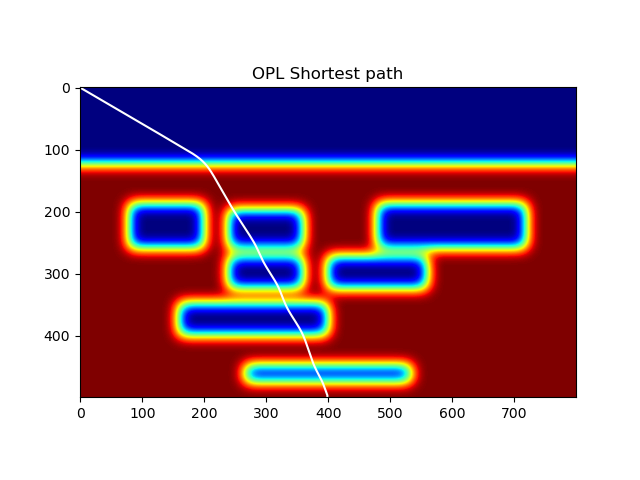
\includegraphics[width=0.45\linewidth]{figs/Ex1/OPL Shortest path.png} &
    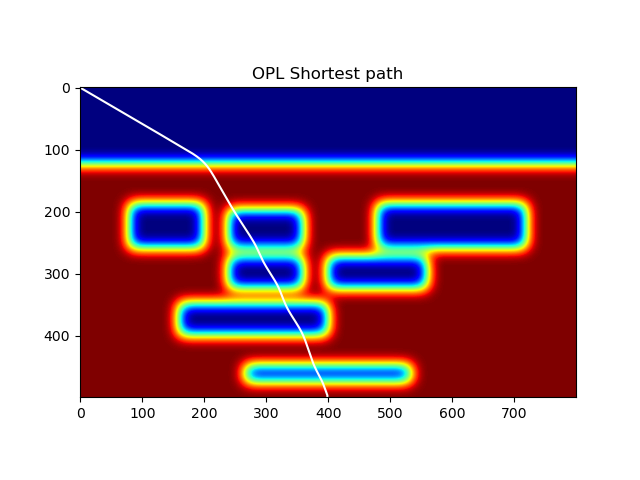
\includegraphics[width=0.45\linewidth]{figs/Ex1/OPL Shortest path.png}
\end{tabular}
\caption{\small left: required path from source to target. right: flipped path from target to source}
\label{fig:OPL}
\end{figure*}

\subsection{}
skip

\clearpage
\subsection{}
Plotting reg-000 original mesh:
\begin{figure*}[h!]
\centering
\begin{tabular}{cc}
    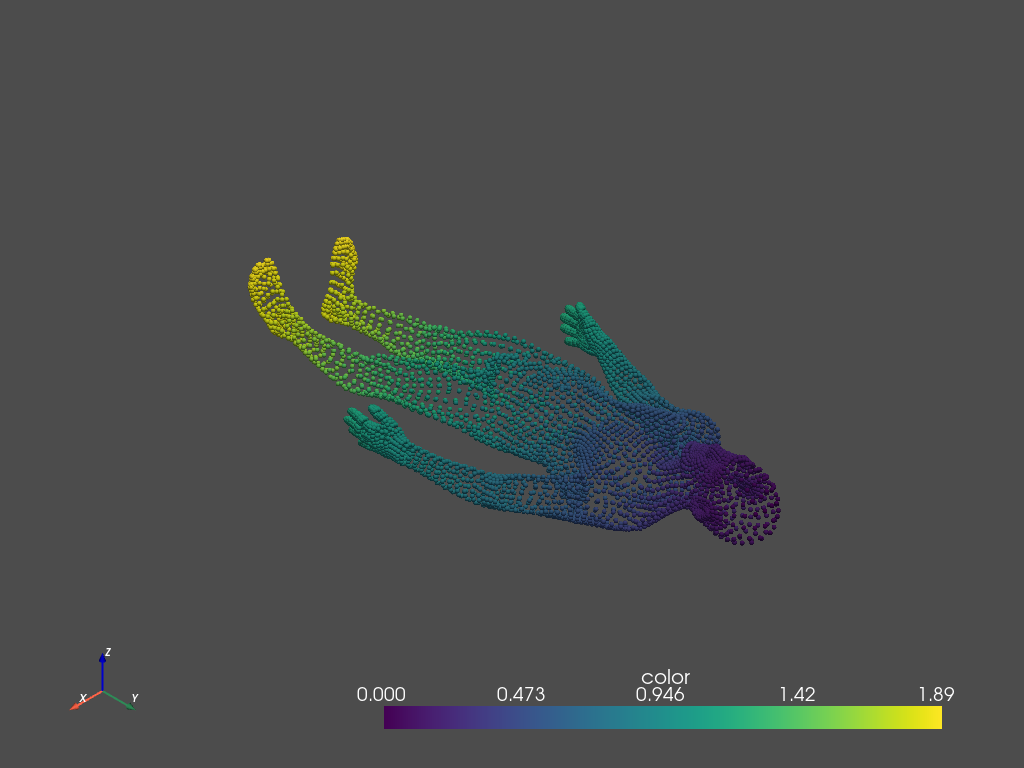
\includegraphics[width=0.45\linewidth]{figs/Ex1/reg_000.png}
\end{tabular}
\caption{\small The original mesh for reg-000}
\end{figure*}

Plotting reg-000 embedding:
\begin{figure*}[h]
\centering
\begin{tabular}{cc}
    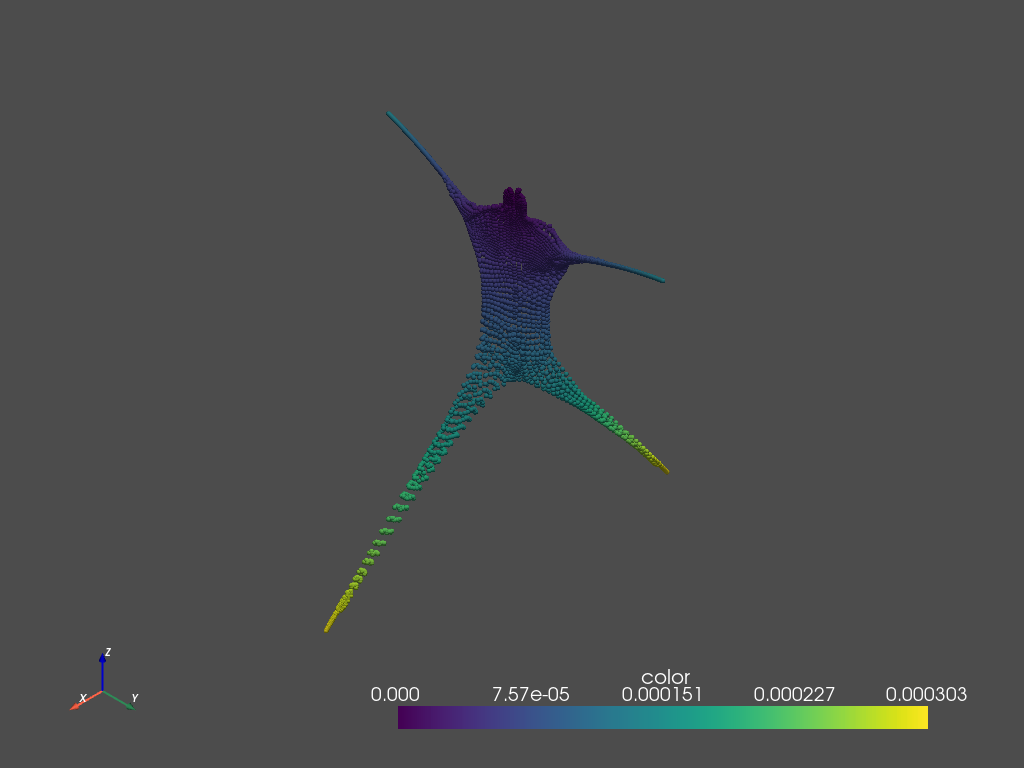
\includegraphics[width=0.45\linewidth]{figs/Ex1/reg_000_MDS.png} &
    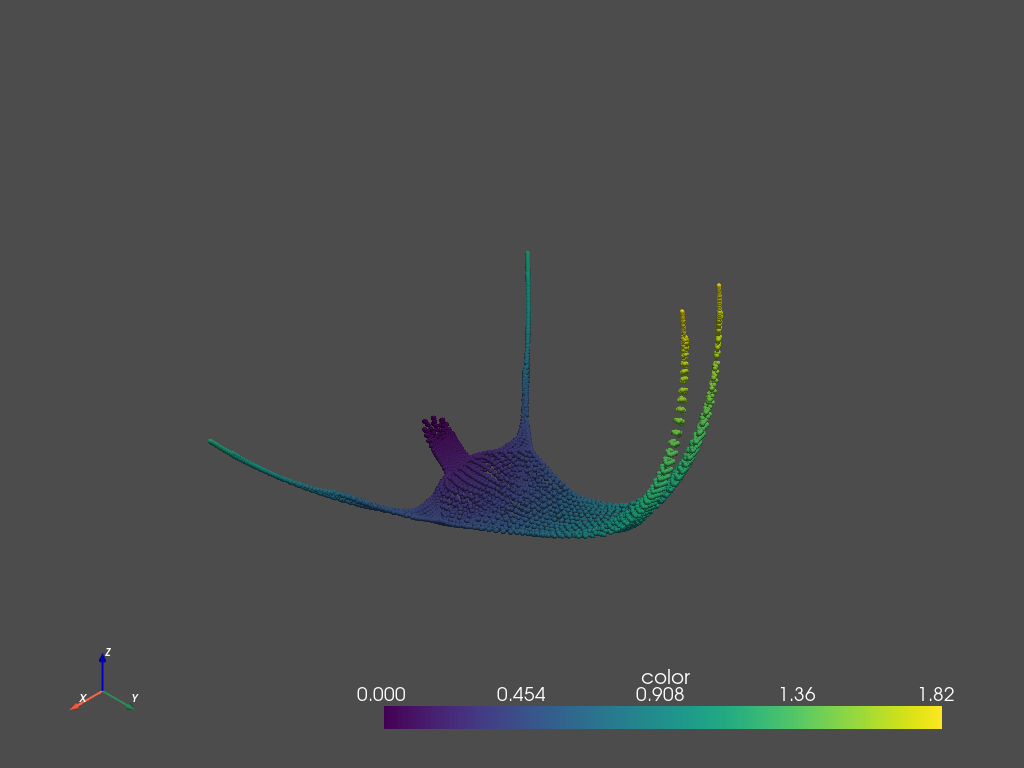
\includegraphics[width=0.45\linewidth]{figs/Ex1/reg_000_Spherical MDS.png}
\end{tabular}
\caption{\small Left: MDS embedding of reg-000. Right: MDS Spherical embedding of reg-000}
\end{figure*}

The error using: \(\epsilon=\|D-\hat{D}\|_F\) is:
\begin{itemize}
\item MDS: 877.7
\item Spherical MDS: 746.8
\end{itemize}

\clearpage
Plotting reg-001 original mesh:
\begin{figure*}[h]
\centering
\begin{tabular}{cc}
    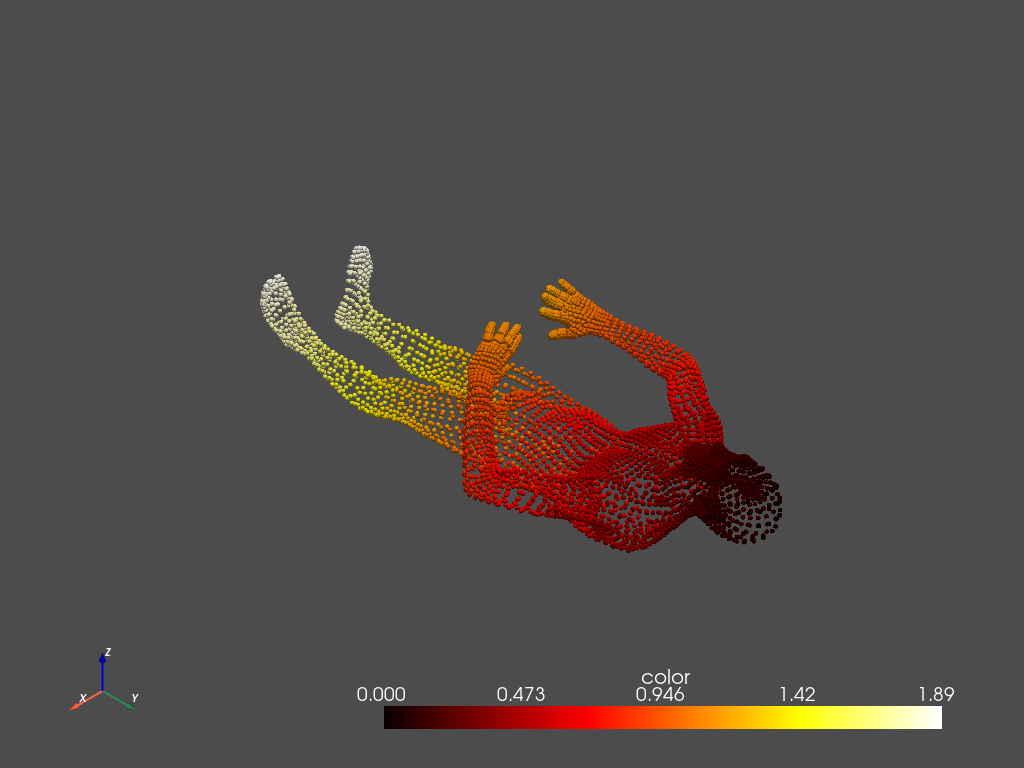
\includegraphics[width=0.45\linewidth]{figs/Ex1/reg_001.png}
\end{tabular}
\caption{\small The original mesh for reg-001}
\end{figure*}

Plotting reg-001 embedding:
\begin{figure*}[h]
\centering
\begin{tabular}{cc}
    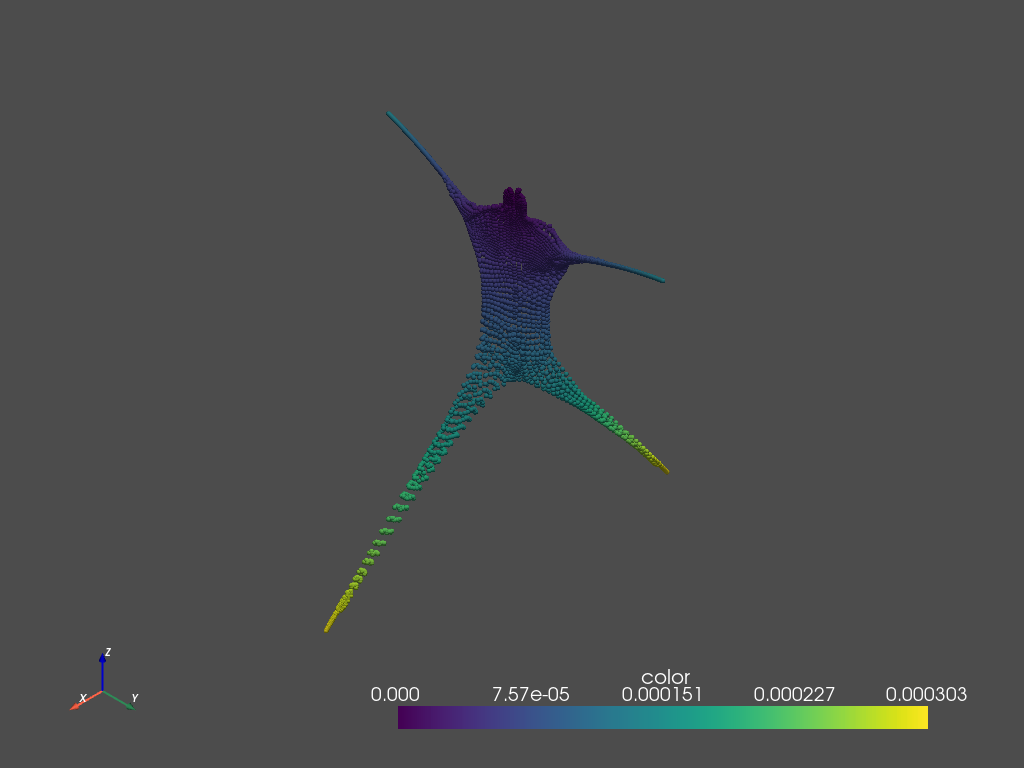
\includegraphics[width=0.45\linewidth]{figs/Ex1/reg_001_MDS.png} &
    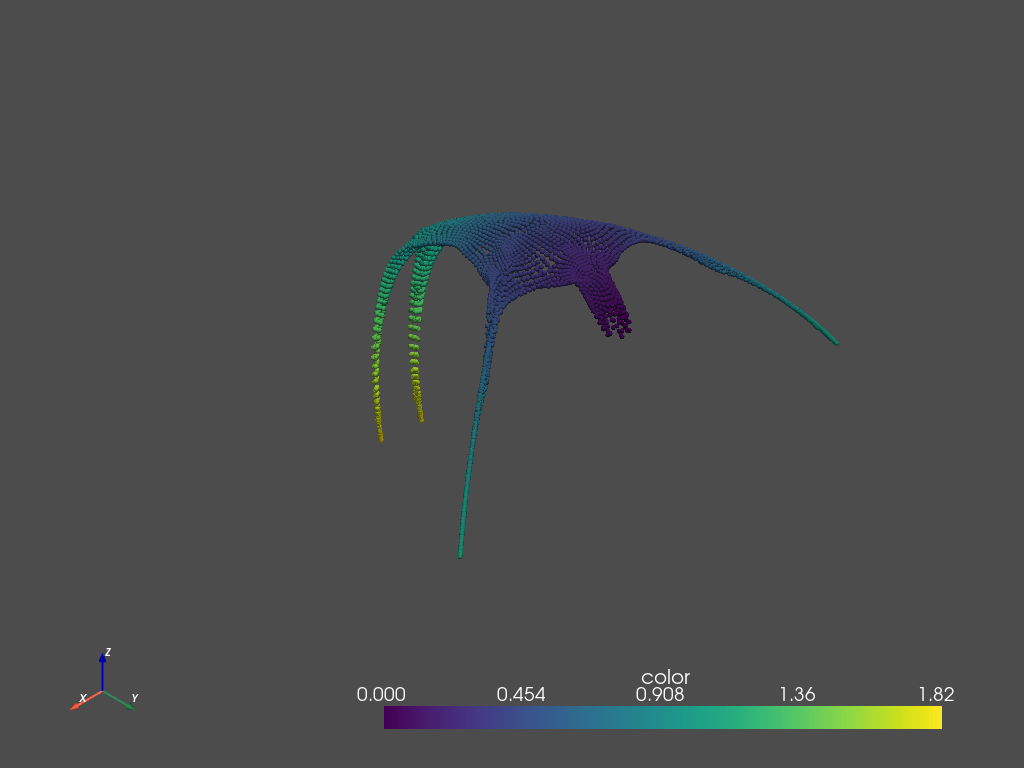
\includegraphics[width=0.45\linewidth]{figs/Ex1/reg_001_Spherical MDS.png}
\end{tabular}
\caption{\small Left: MDS embedding of reg-001. Right: MDS Spherical embedding of reg-001}
\end{figure*}

The error using: \(\epsilon=\|D-\hat{D}\|_F\) is:
\begin{itemize}
\item MDS: 843.6
\item Spherical MDS: 701.5
\end{itemize}

As can be seen from the avatars above is that for both MDS methods the vertices geodesic distances are preserved. For example: the head vertices are close in terms of geodesic distance to each other at the original scan and it also reflect at the embedding presentation. From the other hand, the geodesic distance between the hands and also the legs are pretty big so we can notice the embedding take it into consideration and plots the hand and the legs faraway from each other.  
In addition, we can see the errors between the two methods is in the same order, it means that both of the embedding are achieve good results for dimentionality reduction in this case.

\clearpage
\subsection{}
We sample 1000, 2000, 4000 points.
\begin{figure*}[h]
\centering
\includegraphics[width=0.9\linewidth]{figs/Ex1/reg_000_ReducedMesh by FarestPointSampling.png} 
\caption{\small reg-000 sample with Farest point sampling method}
\end{figure*}
\begin{figure*}[h]
\centering
\includegraphics[width=0.9\linewidth]{figs/Ex1/reg_001_ReducedMesh by FarestPointSampling.png} 
\caption{\small reg-001 sample with Farest point sampling method}
\end{figure*}